\documentclass[letter,french]{report}
\usepackage[T1]{fontenc}
\usepackage[utf8]{inputenc} 
\usepackage{lmodern}
\usepackage{babel}
\usepackage[pdftex]{graphicx}
\usepackage{wasysym}
\usepackage{amsmath,amssymb}



\begin{document}
\title{Devoir 1 IFT 3913}
\author{Ludovic André et Gevrai Jodoin-Tremblay}
\date{Remis le 5 Octobre 2017}
\maketitle

\section*{Introduction}

\subsection*{Description du logiciel}
Ce logiciel affiche une interface usager simple à l'ouverture, très semblable
à l'exemple d'interface usager de l'énoncé du travail pratique. Le bouton "Charger
fichier" ouvre une fenêtre système permettant de sélectionner un fichier .ucd.
Lorsqu'un fichier est choisi, il est \emph{parser} et ses éléments sont affichés dans
les champs correspondants de l'interface.

\subsection*{Ligne de compilation}
Nous avons opté pour un \emph{makefile} histoire de rendre la compilation et l'exécution
la plus facile possible sur les machines du DIRO. Un simple \emph{make} compile
l'entiereté du logiciel et l'exécute. Pour voir les autres options, \emph{make help}
explique les différentes commandes possibles.

\section*{Conception}
Pour notre travail nous avons décidé de diviser notre projet en 3 différents
paquets, comme on le voit dans le diagramme de paquet suivant.
\newline 
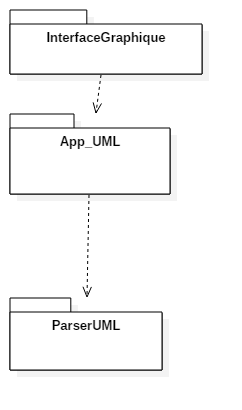
\includegraphics[scale=.3]{DiagrammePaquet.png}

\subsection{Parseur}
Le parseur est inclus dans une seule classe statique, dont la seule méthode
publique \emph{parse} prend une liste de \emph{String} correspondants aux lignes d'un
fichier \emph{.ucd} et renvoit le \emph{UMLModel} correspondant. 

Le \emph{parsing} est majoritairement fait avec des expressions régulières,
principalement parce que la grammaire \emph{BNF} donné dans l'énoncé si
prêtait particulièrement bien. Ainsi, on découpe le texte en de plus en plus
petits tronçons et on créer les objets du paquet \emph{uml} directement.

\subsection{Interface Usager}


\subsection{Représentation des éléments UML}
L'image suivante montre le diagramme de Classe de notre représentation UML.
\newline 
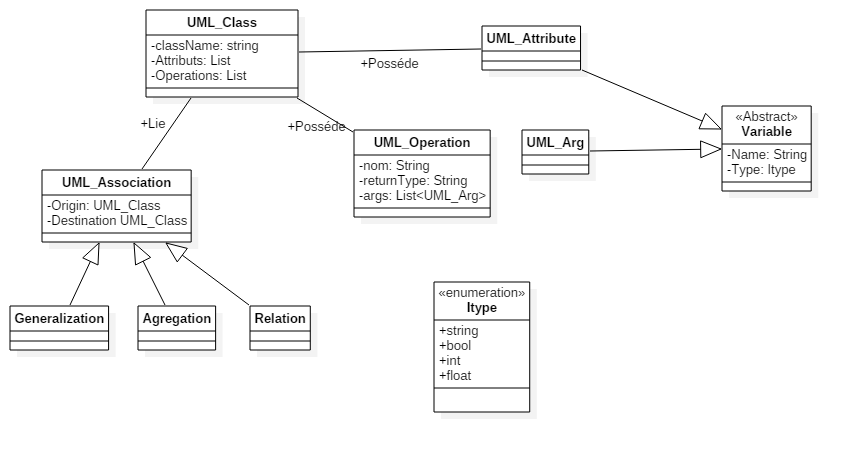
\includegraphics[scale=.3]{DiagrammeClasse.png}

Ainsi, nous avons divisé en plusieurs classe notre représentation des éléments
\emph{UML}. Tout en haut, la classe \emph{UMLModel} contient tout les autres
éléments nécessaires. Nous avons une classe "UML\_Classe" qui représente les
classes \emph{UML}. Ensuite cette classe posséde des opérations et des attributs, qui eux mêmes ont
des 

De l'autre côté on a la
classe "UML\_Association" qui elle a pour unique but de démontrer les liens
entre 2 classes indiqué dans le diagramme UML.
\newline
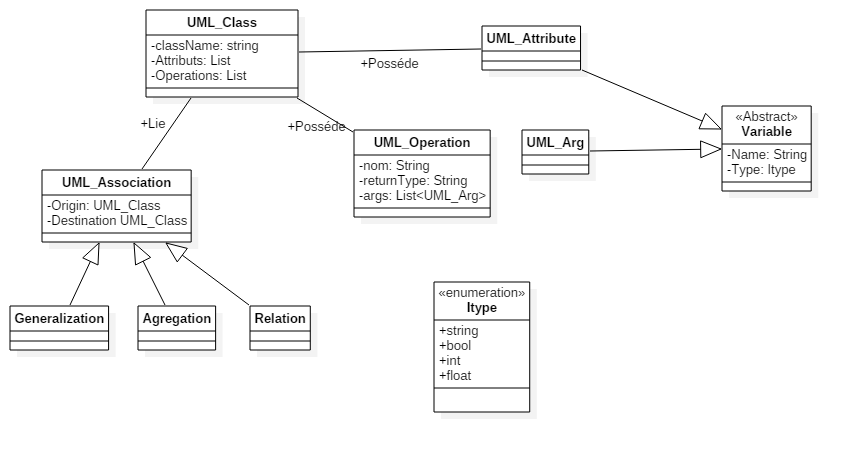
\includegraphics[scale=.4]{DiagrammeClasse.png}

\section*{Implantation}

\subsection{Parseur}
Le parseur est inclus dans une seule classe statique, dont la seule méthode
publique \emph{parse} prend une liste de \emph{String} correspondants aux lignes d'un
fichier \emph{.ucd} et renvoit le \emph{UMLModel} correspondant. 

Le \emph{parsing} est majoritairement fait avec des expressions régulières,
principalement parce que la grammaire \emph{BNF} donné dans l'énoncé si
prêtait particulièrement bien. Ainsi, on découpe le texte en de plus en plus
petits tronçons et on créer les objets du paquet \emph{uml} directement.

\section*{Problèmes rencontrés}

\section*{Développement futur}
Il serait très utile de pouvoir modifier un modèle UML directement à partir de l'interface,
et permette l'exportation vers un fichier /.ucd/.



\section*{Exécution du code java}

\end{document}
